\documentclass[]{article}
\usepackage{lmodern}
\usepackage{amssymb,amsmath}
\usepackage{ifxetex,ifluatex}
\usepackage{fixltx2e} % provides \textsubscript
\ifnum 0\ifxetex 1\fi\ifluatex 1\fi=0 % if pdftex
  \usepackage[T1]{fontenc}
  \usepackage[utf8]{inputenc}
\else % if luatex or xelatex
  \ifxetex
    \usepackage{mathspec}
  \else
    \usepackage{fontspec}
  \fi
  \defaultfontfeatures{Ligatures=TeX,Scale=MatchLowercase}
\fi
% use upquote if available, for straight quotes in verbatim environments
\IfFileExists{upquote.sty}{\usepackage{upquote}}{}
% use microtype if available
\IfFileExists{microtype.sty}{%
\usepackage{microtype}
\UseMicrotypeSet[protrusion]{basicmath} % disable protrusion for tt fonts
}{}
\usepackage[margin=1in]{geometry}
\usepackage{hyperref}
\hypersetup{unicode=true,
            pdftitle={Beer Analysis},
            pdfauthor={Robert Hazell},
            pdfborder={0 0 0},
            breaklinks=true}
\urlstyle{same}  % don't use monospace font for urls
\usepackage{color}
\usepackage{fancyvrb}
\newcommand{\VerbBar}{|}
\newcommand{\VERB}{\Verb[commandchars=\\\{\}]}
\DefineVerbatimEnvironment{Highlighting}{Verbatim}{commandchars=\\\{\}}
% Add ',fontsize=\small' for more characters per line
\usepackage{framed}
\definecolor{shadecolor}{RGB}{248,248,248}
\newenvironment{Shaded}{\begin{snugshade}}{\end{snugshade}}
\newcommand{\AlertTok}[1]{\textcolor[rgb]{0.94,0.16,0.16}{#1}}
\newcommand{\AnnotationTok}[1]{\textcolor[rgb]{0.56,0.35,0.01}{\textbf{\textit{#1}}}}
\newcommand{\AttributeTok}[1]{\textcolor[rgb]{0.77,0.63,0.00}{#1}}
\newcommand{\BaseNTok}[1]{\textcolor[rgb]{0.00,0.00,0.81}{#1}}
\newcommand{\BuiltInTok}[1]{#1}
\newcommand{\CharTok}[1]{\textcolor[rgb]{0.31,0.60,0.02}{#1}}
\newcommand{\CommentTok}[1]{\textcolor[rgb]{0.56,0.35,0.01}{\textit{#1}}}
\newcommand{\CommentVarTok}[1]{\textcolor[rgb]{0.56,0.35,0.01}{\textbf{\textit{#1}}}}
\newcommand{\ConstantTok}[1]{\textcolor[rgb]{0.00,0.00,0.00}{#1}}
\newcommand{\ControlFlowTok}[1]{\textcolor[rgb]{0.13,0.29,0.53}{\textbf{#1}}}
\newcommand{\DataTypeTok}[1]{\textcolor[rgb]{0.13,0.29,0.53}{#1}}
\newcommand{\DecValTok}[1]{\textcolor[rgb]{0.00,0.00,0.81}{#1}}
\newcommand{\DocumentationTok}[1]{\textcolor[rgb]{0.56,0.35,0.01}{\textbf{\textit{#1}}}}
\newcommand{\ErrorTok}[1]{\textcolor[rgb]{0.64,0.00,0.00}{\textbf{#1}}}
\newcommand{\ExtensionTok}[1]{#1}
\newcommand{\FloatTok}[1]{\textcolor[rgb]{0.00,0.00,0.81}{#1}}
\newcommand{\FunctionTok}[1]{\textcolor[rgb]{0.00,0.00,0.00}{#1}}
\newcommand{\ImportTok}[1]{#1}
\newcommand{\InformationTok}[1]{\textcolor[rgb]{0.56,0.35,0.01}{\textbf{\textit{#1}}}}
\newcommand{\KeywordTok}[1]{\textcolor[rgb]{0.13,0.29,0.53}{\textbf{#1}}}
\newcommand{\NormalTok}[1]{#1}
\newcommand{\OperatorTok}[1]{\textcolor[rgb]{0.81,0.36,0.00}{\textbf{#1}}}
\newcommand{\OtherTok}[1]{\textcolor[rgb]{0.56,0.35,0.01}{#1}}
\newcommand{\PreprocessorTok}[1]{\textcolor[rgb]{0.56,0.35,0.01}{\textit{#1}}}
\newcommand{\RegionMarkerTok}[1]{#1}
\newcommand{\SpecialCharTok}[1]{\textcolor[rgb]{0.00,0.00,0.00}{#1}}
\newcommand{\SpecialStringTok}[1]{\textcolor[rgb]{0.31,0.60,0.02}{#1}}
\newcommand{\StringTok}[1]{\textcolor[rgb]{0.31,0.60,0.02}{#1}}
\newcommand{\VariableTok}[1]{\textcolor[rgb]{0.00,0.00,0.00}{#1}}
\newcommand{\VerbatimStringTok}[1]{\textcolor[rgb]{0.31,0.60,0.02}{#1}}
\newcommand{\WarningTok}[1]{\textcolor[rgb]{0.56,0.35,0.01}{\textbf{\textit{#1}}}}
\usepackage{graphicx,grffile}
\makeatletter
\def\maxwidth{\ifdim\Gin@nat@width>\linewidth\linewidth\else\Gin@nat@width\fi}
\def\maxheight{\ifdim\Gin@nat@height>\textheight\textheight\else\Gin@nat@height\fi}
\makeatother
% Scale images if necessary, so that they will not overflow the page
% margins by default, and it is still possible to overwrite the defaults
% using explicit options in \includegraphics[width, height, ...]{}
\setkeys{Gin}{width=\maxwidth,height=\maxheight,keepaspectratio}
\IfFileExists{parskip.sty}{%
\usepackage{parskip}
}{% else
\setlength{\parindent}{0pt}
\setlength{\parskip}{6pt plus 2pt minus 1pt}
}
\setlength{\emergencystretch}{3em}  % prevent overfull lines
\providecommand{\tightlist}{%
  \setlength{\itemsep}{0pt}\setlength{\parskip}{0pt}}
\setcounter{secnumdepth}{0}
% Redefines (sub)paragraphs to behave more like sections
\ifx\paragraph\undefined\else
\let\oldparagraph\paragraph
\renewcommand{\paragraph}[1]{\oldparagraph{#1}\mbox{}}
\fi
\ifx\subparagraph\undefined\else
\let\oldsubparagraph\subparagraph
\renewcommand{\subparagraph}[1]{\oldsubparagraph{#1}\mbox{}}
\fi

%%% Use protect on footnotes to avoid problems with footnotes in titles
\let\rmarkdownfootnote\footnote%
\def\footnote{\protect\rmarkdownfootnote}

%%% Change title format to be more compact
\usepackage{titling}

% Create subtitle command for use in maketitle
\newcommand{\subtitle}[1]{
  \posttitle{
    \begin{center}\large#1\end{center}
    }
}

\setlength{\droptitle}{-2em}

  \title{Beer Analysis}
    \pretitle{\vspace{\droptitle}\centering\huge}
  \posttitle{\par}
    \author{Robert Hazell}
    \preauthor{\centering\large\emph}
  \postauthor{\par}
      \predate{\centering\large\emph}
  \postdate{\par}
    \date{2/27/2019}

\usepackage{booktabs}
\usepackage{longtable}
\usepackage{array}
\usepackage{multirow}
\usepackage{wrapfig}
\usepackage{float}
\usepackage{colortbl}
\usepackage{pdflscape}
\usepackage{tabu}
\usepackage{threeparttable}
\usepackage{threeparttablex}
\usepackage[normalem]{ulem}
\usepackage{makecell}
\usepackage{xcolor}

\begin{document}
\maketitle

\hypertarget{xyz-brewery-proposal}{%
\subsection{XYZ Brewery Proposal}\label{xyz-brewery-proposal}}

\hypertarget{introduction}{%
\subsubsection{Introduction}\label{introduction}}

According to
\href{http://fortune.com/2018/03/27/craft-beer-2017-sales/}{Fortune} the
US Craft Brew industry was worth \$26 billion dollars in 2017, an
increase of \$6.2 billion since 2015. While the pace of growth is
slowing, opportunity is still large. It's known that craft beer drinkers
tend to support local independent breweries, and consumers are becoming
more selective. Furthermore there is
\href{https://www.grandviewresearch.com/press-release/global-craft-beer-market}{rising
demand} for low alcohol by volume (ABV) and flavored beer. Each market
share of .5\% is equivalent to \$130 million in revenue.

As a start-up XYZ faces a saturated market. There are two purposes of
this research, first of which is to examine the current landscape and
scope out under-served areas in the US where few breweries exist. Second
is to understand what beer preference(s) would be most profitable should
a brewery (or breweries) be built.
\href{https://www.craftbeer.com/craft-beer-muses/craft-beer-by-the-numbers}{Craftbeer}
reports that four key statistics are used to describe craft beers:

\textbf{1)} Serving size

\textbf{2)} International Bitterness Units (IBU): the bitterness element
of a beer's flavor

\textbf{3)} Alcohol by Volume (ABV): higher values increase the
complexity and flavor of the beer

\textbf{4)} Original Gravity / Final Gravity: factors which affect ABV
and sensory intensity

This report will focus on IBU and ABV. It will also integrate data on
drinking consumption by state to clarify each state's drinking behavior.

\hypertarget{competitive-landscape-how-many-craft-breweries-are-currently-producing-in-the-us}{%
\subsubsection{Competitive Landscape: How many craft breweries are
currently producing in the
US?}\label{competitive-landscape-how-many-craft-breweries-are-currently-producing-in-the-us}}

The relevant datasets are \emph{Beers.csv} and \emph{Breweries.csv}.
Each will be loaded each into R after setting a working a directory.

\begin{Shaded}
\begin{Highlighting}[]
\KeywordTok{setwd}\NormalTok{(}\StringTok{"/Users/roberthazell/Desktop/DataScience@SMU/DoingDataScience/CaseStudy1"}\NormalTok{)}
\NormalTok{beers <-}\StringTok{ }\KeywordTok{read.csv}\NormalTok{(}\StringTok{"beers.csv"}\NormalTok{)}
\NormalTok{brewers <-}\StringTok{ }\KeywordTok{read.csv}\NormalTok{(}\StringTok{"breweries.csv"}\NormalTok{)}
\end{Highlighting}
\end{Shaded}

The total number of breweries can be found be inspecting the
\texttt{State} column of \texttt{brewers}. There are 558 unique
breweries in the U.S.

\begin{Shaded}
\begin{Highlighting}[]
\KeywordTok{length}\NormalTok{(brewers}\OperatorTok{$}\NormalTok{State)}
\end{Highlighting}
\end{Shaded}

\begin{verbatim}
[1] 558
\end{verbatim}

\hypertarget{combining-data-sources-to-better-understand-us-craft-brewing}{%
\subsubsection{Combining data sources to better understand US craft
brewing}\label{combining-data-sources-to-better-understand-us-craft-brewing}}

By merging the \emph{beers} and \emph{brewers} datasets, a more complete
picture of the US beer landscape is possible. Each dataset will be
merged on their common \emph{id} columns. This is \texttt{Brewery\_id}
and \texttt{Brew\_ID}, which are equivalent.

\begin{Shaded}
\begin{Highlighting}[]
\NormalTok{Brewtot <-}\StringTok{ }\KeywordTok{merge}\NormalTok{(beers, brewers, }\DataTypeTok{by.x =} \StringTok{"Brewery_id"}\NormalTok{, }\DataTypeTok{by.y =} \StringTok{"Brew_ID"}\NormalTok{)}
\end{Highlighting}
\end{Shaded}

Here is a look at the first six rows of the merged data, as there are
over 2000 rows in the dataset.

\begin{Shaded}
\begin{Highlighting}[]
\KeywordTok{nrow}\NormalTok{(Brewtot) }\CommentTok{# number of rows}
\end{Highlighting}
\end{Shaded}

\begin{verbatim}
[1] 2410
\end{verbatim}

\begin{Shaded}
\begin{Highlighting}[]
\KeywordTok{head}\NormalTok{(Brewtot) }\CommentTok{# first six observations}
\end{Highlighting}
\end{Shaded}

\begin{verbatim}
  Brewery_id        Name.x Beer_ID   ABV IBU
1          1  Get Together    2692 0.045  50
2          1 Maggie's Leap    2691 0.049  26
3          1    Wall's End    2690 0.048  19
4          1       Pumpion    2689 0.060  38
5          1    Stronghold    2688 0.060  25
6          1   Parapet ESB    2687 0.056  47
                                Style Ounces             Name.y
1                        American IPA     16 NorthGate Brewing 
2                  Milk / Sweet Stout     16 NorthGate Brewing 
3                   English Brown Ale     16 NorthGate Brewing 
4                         Pumpkin Ale     16 NorthGate Brewing 
5                     American Porter     16 NorthGate Brewing 
6 Extra Special / Strong Bitter (ESB)     16 NorthGate Brewing 
         City State
1 Minneapolis    MN
2 Minneapolis    MN
3 Minneapolis    MN
4 Minneapolis    MN
5 Minneapolis    MN
6 Minneapolis    MN
\end{verbatim}

Renaming \texttt{Name.x} and \texttt{Name.y} increases clarity. They
will represent the \texttt{Beer} name and \texttt{Brewer}, respectively.

\begin{Shaded}
\begin{Highlighting}[]
\KeywordTok{colnames}\NormalTok{(Brewtot)[}\KeywordTok{c}\NormalTok{(}\DecValTok{2}\NormalTok{,}\DecValTok{8}\NormalTok{)] =}\StringTok{ }\KeywordTok{c}\NormalTok{(}\StringTok{"Beer"}\NormalTok{, }\StringTok{"Brewer"}\NormalTok{)}
\end{Highlighting}
\end{Shaded}

\hypertarget{missing-information}{%
\subsubsection{Missing Information}\label{missing-information}}

Before further analyzing the data it's best to see if any missing values
(\texttt{NA}) exist.

\begin{Shaded}
\begin{Highlighting}[]
\NormalTok{Brewtot_Missing <-}\StringTok{ }\KeywordTok{sapply}\NormalTok{(Brewtot, }\ControlFlowTok{function}\NormalTok{(x) }\KeywordTok{sum}\NormalTok{(}\KeywordTok{is.na}\NormalTok{(x)))}
\NormalTok{Brewtot_Missing}
\end{Highlighting}
\end{Shaded}

\begin{verbatim}
Brewery_id       Beer    Beer_ID        ABV        IBU      Style 
         0          0          0         62       1005          0 
    Ounces     Brewer       City      State 
         0          0          0          0 
\end{verbatim}

On the two important metrics \texttt{ABV} and \texttt{IBU}, there are 62
and 1005 missing values respectively. This means our data may have
limitations, namely it may not be completely representative of the
entire brewing industry. As will be shown later, however, there is much
utility still.

\hypertarget{market-saturation}{%
\subsubsection{Market Saturation}\label{market-saturation}}

In determining where to build any brewery, it's advisable to avoid
states with many breweries already. To that end, the merged dataset
\texttt{Brewtot} can be used to summarize the total number of unique
brews and brewers per state.

\begin{Shaded}
\begin{Highlighting}[]
\KeywordTok{library}\NormalTok{(dplyr)}
\KeywordTok{library}\NormalTok{(kableExtra)}

\NormalTok{beer_landscape <-}\StringTok{ }\NormalTok{Brewtot }\OperatorTok\StringTok{ }\KeywordTok{group_by}\NormalTok{(State) }\OperatorTok\StringTok{ }\KeywordTok{summarise}\NormalTok{(}\DataTypeTok{Beers =} \KeywordTok{length}\NormalTok{(Beer)) }\OperatorTok\StringTok{ }\KeywordTok{cbind}\NormalTok{(brewers }\OperatorTok\StringTok{ }\KeywordTok{group_by}\NormalTok{(State) }\OperatorTok\StringTok{ }\KeywordTok{summarise}\NormalTok{(}\StringTok{`}\DataTypeTok{Total Brewers}\StringTok{`}\NormalTok{ =}\StringTok{ }\KeywordTok{length}\NormalTok{(State)) }\OperatorTok\StringTok{ }\KeywordTok{select}\NormalTok{(}\StringTok{`}\DataTypeTok{Total Brewers}\StringTok{`}\NormalTok{)) }\OperatorTok\StringTok{ }\KeywordTok{arrange}\NormalTok{(}\KeywordTok{desc}\NormalTok{(}\StringTok{`}\DataTypeTok{Total Brewers}\StringTok{`}\NormalTok{)) }\OperatorTok\StringTok{ }\KeywordTok{data.frame}\NormalTok{()}
\NormalTok{beer_landscape}\OperatorTok{$}\NormalTok{State <-}\StringTok{ }\KeywordTok{trimws}\NormalTok{(beer_landscape}\OperatorTok{$}\NormalTok{State)}

\KeywordTok{str}\NormalTok{(beer_landscape)}
\end{Highlighting}
\end{Shaded}

\begin{verbatim}
'data.frame':   51 obs. of  3 variables:
 $ State        : chr  "CO" "CA" "MI" "OR" ...
 $ Beers        : int  265 183 162 125 130 100 82 68 139 87 ...
 $ Total.Brewers: int  47 39 32 29 28 25 23 23 22 20 ...
\end{verbatim}

\begin{Shaded}
\begin{Highlighting}[]
\KeywordTok{kable}\NormalTok{(beer_landscape, }\DataTypeTok{align =} \KeywordTok{rep}\NormalTok{(}\StringTok{'c'}\NormalTok{,}\DecValTok{3}\NormalTok{)) }\OperatorTok\StringTok{ }\KeywordTok{kable_styling}\NormalTok{(}\DataTypeTok{bootstrap_options =} \StringTok{"striped"}\NormalTok{, }\DataTypeTok{full_width =}\NormalTok{ F)}
\end{Highlighting}
\end{Shaded}

\begin{table}[H]
\centering
\begin{tabular}{c|c|c}
\hline
State & Beers & Total.Brewers\\
\hline
CO & 265 & 47\\
\hline
CA & 183 & 39\\
\hline
MI & 162 & 32\\
\hline
OR & 125 & 29\\
\hline
TX & 130 & 28\\
\hline
PA & 100 & 25\\
\hline
MA & 82 & 23\\
\hline
WA & 68 & 23\\
\hline
IN & 139 & 22\\
\hline
WI & 87 & 20\\
\hline
NC & 59 & 19\\
\hline
IL & 91 & 18\\
\hline
NY & 74 & 16\\
\hline
VA & 40 & 16\\
\hline
FL & 58 & 15\\
\hline
OH & 49 & 15\\
\hline
MN & 55 & 12\\
\hline
AZ & 47 & 11\\
\hline
VT & 27 & 10\\
\hline
ME & 27 & 9\\
\hline
MO & 42 & 9\\
\hline
MT & 40 & 9\\
\hline
CT & 27 & 8\\
\hline
AK & 25 & 7\\
\hline
GA & 16 & 7\\
\hline
MD & 21 & 7\\
\hline
OK & 19 & 6\\
\hline
IA & 30 & 5\\
\hline
ID & 30 & 5\\
\hline
LA & 19 & 5\\
\hline
NE & 25 & 5\\
\hline
RI & 27 & 5\\
\hline
HI & 27 & 4\\
\hline
KY & 21 & 4\\
\hline
NM & 14 & 4\\
\hline
SC & 14 & 4\\
\hline
UT & 26 & 4\\
\hline
WY & 15 & 4\\
\hline
AL & 10 & 3\\
\hline
KS & 23 & 3\\
\hline
NH & 8 & 3\\
\hline
NJ & 8 & 3\\
\hline
TN & 6 & 3\\
\hline
AR & 5 & 2\\
\hline
DE & 2 & 2\\
\hline
MS & 11 & 2\\
\hline
NV & 11 & 2\\
\hline
DC & 8 & 1\\
\hline
ND & 3 & 1\\
\hline
SD & 7 & 1\\
\hline
WV & 2 & 1\\
\hline
\end{tabular}
\end{table}

From this we see Colorado has the highest number of beers and breweries.
So XYZ should probably avoid that state!

\hypertarget{general-differences-in-beer-characteristics}{%
\subsubsection{General Differences in Beer
Characteristics}\label{general-differences-in-beer-characteristics}}

Before looking at state and regional differences in IBU and ABV, an
overall view of their distribution is helpful.

\begin{Shaded}
\begin{Highlighting}[]
\KeywordTok{hist}\NormalTok{(Brewtot}\OperatorTok{$}\NormalTok{ABV, }\DataTypeTok{main=}\StringTok{"Distribution of ABV"}\NormalTok{, }\DataTypeTok{breaks=}\DecValTok{20}\NormalTok{, }\DataTypeTok{xlab=}\StringTok{"Alcohol by Volume"}\NormalTok{, }\DataTypeTok{border=}\StringTok{"black"}\NormalTok{, }\DataTypeTok{col=}\StringTok{"steel blue"}\NormalTok{, }\DataTypeTok{xlim=}\KeywordTok{c}\NormalTok{(.}\DecValTok{02}\NormalTok{,.}\DecValTok{13}\NormalTok{)) }
\end{Highlighting}
\end{Shaded}

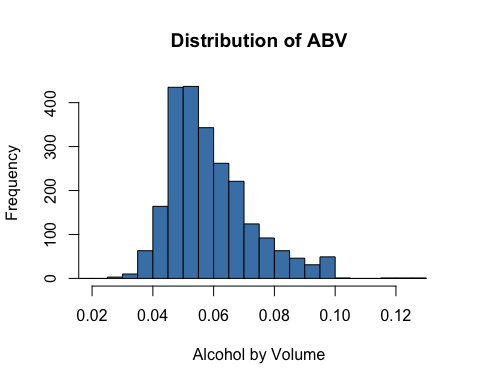
\includegraphics{BeerAnalysis_files/figure-latex/unnamed-chunk-9-1.pdf}

\begin{Shaded}
\begin{Highlighting}[]
\KeywordTok{hist}\NormalTok{(Brewtot}\OperatorTok{$}\NormalTok{IBU, }\DataTypeTok{main=}\StringTok{"Distribution of IBU"}\NormalTok{, }\DataTypeTok{breaks=}\DecValTok{20}\NormalTok{, }\DataTypeTok{xlab=}\StringTok{"International Bitterness Units"}\NormalTok{, }\DataTypeTok{border=}\StringTok{"black"}\NormalTok{, }\DataTypeTok{col=}\StringTok{"dark red"}\NormalTok{, }\DataTypeTok{xlim=}\KeywordTok{c}\NormalTok{(}\DecValTok{0}\NormalTok{,}\DecValTok{100}\NormalTok{))}
\end{Highlighting}
\end{Shaded}

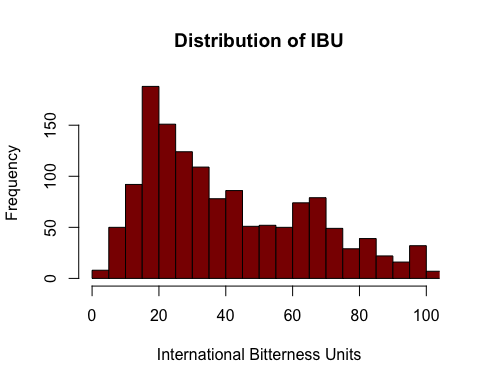
\includegraphics{BeerAnalysis_files/figure-latex/unnamed-chunk-9-2.pdf}

ABV is mostly centered around .05, with a moderate right skew. On the
other hand, IBU has a strong right skew. In spite of the peak at
\textasciitilde{} 20 IBU, a lot of beers have a bitter side, too.

\hypertarget{state-differences-in-beer-characteristics}{%
\subsubsection{State Differences in Beer
Characteristics}\label{state-differences-in-beer-characteristics}}

Perhaps ABV and/or IBU stabilizes when \emph{median} values are
examined. That data needs gathering first.

\begin{Shaded}
\begin{Highlighting}[]
\NormalTok{alcohol_and_bitterness <-}\StringTok{ }\NormalTok{Brewtot }\OperatorTok\StringTok{ }\KeywordTok{group_by}\NormalTok{(State) }\OperatorTok\StringTok{ }
\StringTok{  }\KeywordTok{summarise}\NormalTok{(}\DataTypeTok{MedianAlcohol =} \KeywordTok{median}\NormalTok{(ABV, }\DataTypeTok{na.rm =}\NormalTok{ T), }\DataTypeTok{MedianBitter =} \KeywordTok{median}\NormalTok{(IBU, }\DataTypeTok{na.rm =}\NormalTok{ T))}
\end{Highlighting}
\end{Shaded}

South Dakota has absolutely no information on bitterness for their
beers, so it will be deleted.

\begin{Shaded}
\begin{Highlighting}[]
\NormalTok{alcohol_and_bitterness <-}\StringTok{ }\NormalTok{alcohol_and_bitterness[}\OperatorTok{-}\DecValTok{42}\NormalTok{,]}
\end{Highlighting}
\end{Shaded}

Here are the median distributions for IBU and ABV by state.

\begin{Shaded}
\begin{Highlighting}[]
\KeywordTok{library}\NormalTok{(ggplot2)}

\KeywordTok{ggplot}\NormalTok{(alcohol_and_bitterness) }\OperatorTok{+}\StringTok{ }
\StringTok{  }\KeywordTok{geom_col}\NormalTok{(}\KeywordTok{aes}\NormalTok{(}\DataTypeTok{x =} \KeywordTok{reorder}\NormalTok{(State, MedianAlcohol), }\DataTypeTok{y =}\NormalTok{ MedianAlcohol), }\DataTypeTok{fill =} \StringTok{'steel blue'}\NormalTok{) }\OperatorTok{+}\StringTok{ }\KeywordTok{coord_flip}\NormalTok{() }\OperatorTok{+}\StringTok{ }\KeywordTok{ylab}\NormalTok{(}\StringTok{"Median ABV"}\NormalTok{) }\OperatorTok{+}\StringTok{ }\KeywordTok{xlab}\NormalTok{(}\StringTok{"State"}\NormalTok{) }\OperatorTok{+}\StringTok{ }\KeywordTok{ggtitle}\NormalTok{(}\StringTok{"Median Alcohol Volume by State"}\NormalTok{) }\OperatorTok{+}\StringTok{ }\KeywordTok{theme}\NormalTok{(}\DataTypeTok{plot.title =} \KeywordTok{element_text}\NormalTok{(}\DataTypeTok{hjust =} \FloatTok{0.5}\NormalTok{))}
\end{Highlighting}
\end{Shaded}

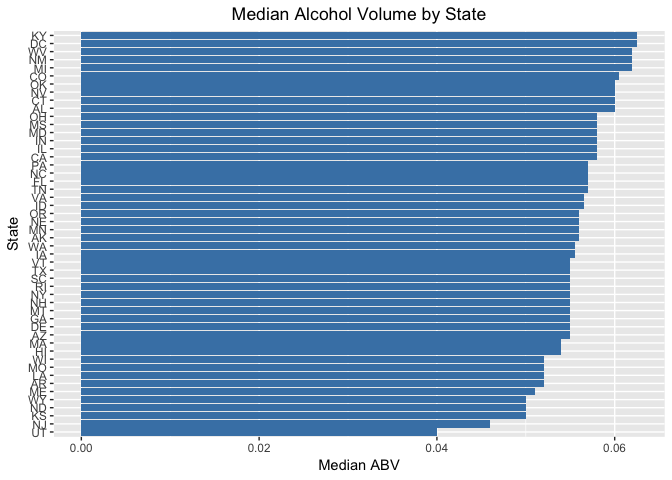
\includegraphics{BeerAnalysis_files/figure-latex/unnamed-chunk-12-1.pdf}

\begin{Shaded}
\begin{Highlighting}[]
\KeywordTok{ggplot}\NormalTok{(alcohol_and_bitterness) }\OperatorTok{+}\StringTok{ }
\StringTok{  }\KeywordTok{geom_col}\NormalTok{(}\KeywordTok{aes}\NormalTok{(}\DataTypeTok{x =} \KeywordTok{reorder}\NormalTok{(State, MedianBitter), }\DataTypeTok{y =}\NormalTok{ MedianBitter), }\DataTypeTok{fill =} \StringTok{'orange'}\NormalTok{) }\OperatorTok{+}\StringTok{ }\KeywordTok{coord_flip}\NormalTok{() }\OperatorTok{+}\StringTok{ }\KeywordTok{ylab}\NormalTok{(}\StringTok{"Median IBU"}\NormalTok{) }\OperatorTok{+}\StringTok{ }\KeywordTok{xlab}\NormalTok{(}\StringTok{"State"}\NormalTok{) }\OperatorTok{+}\StringTok{ }\KeywordTok{ggtitle}\NormalTok{(}\StringTok{"Median Beer Bitterness by State"}\NormalTok{) }\OperatorTok{+}\StringTok{  }\KeywordTok{theme}\NormalTok{(}\DataTypeTok{plot.title =} \KeywordTok{element_text}\NormalTok{(}\DataTypeTok{hjust =} \FloatTok{0.5}\NormalTok{))}
\end{Highlighting}
\end{Shaded}

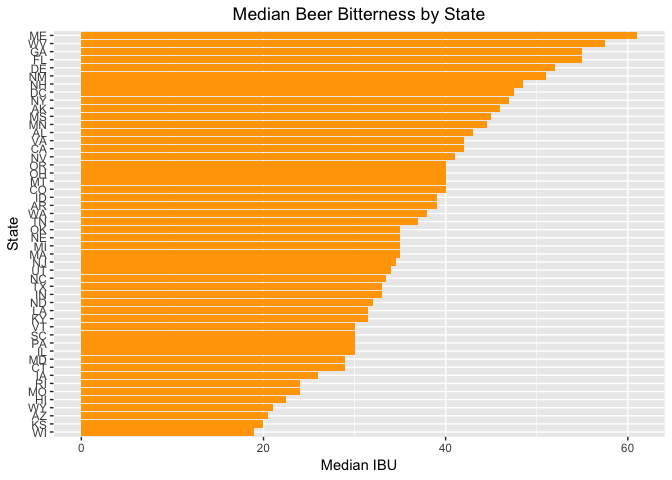
\includegraphics{BeerAnalysis_files/figure-latex/unnamed-chunk-12-2.pdf}

This confirms the assumption that at least one of the variables
stabilize when median values are examined (in this case, ABV).
Nevertheless, median IBU still displays significant variation, with
Maine featuring a median IBU more than triple that of Wisconsin's.

\hypertarget{regional-differences-in-beer-characteristics}{%
\subsubsection{Regional Differences in Beer
Characteristics}\label{regional-differences-in-beer-characteristics}}

What if median bitterness of beer brewed different at a regional level?
Let's test this claim.

First, define the four US regions according to the
\href{https://www.businessinsider.com/regions-of-united-states-2018-5}{Census
Bureau's} standards.

\begin{Shaded}
\begin{Highlighting}[]
\NormalTok{northeast =}\StringTok{ }\KeywordTok{c}\NormalTok{(}\StringTok{'ME'}\NormalTok{, }\StringTok{'NH'}\NormalTok{, }\StringTok{'VT'}\NormalTok{, }\StringTok{'MA'}\NormalTok{, }\StringTok{'RI'}\NormalTok{, }\StringTok{'CT'}\NormalTok{, }\StringTok{'NY'}\NormalTok{, }\StringTok{'NJ'}\NormalTok{, }\StringTok{'PA'}\NormalTok{)}
\NormalTok{midwest =}\StringTok{ }\KeywordTok{c}\NormalTok{(}\StringTok{'ND'}\NormalTok{, }\StringTok{'SD'}\NormalTok{, }\StringTok{'NE'}\NormalTok{, }\StringTok{'KS'}\NormalTok{, }\StringTok{'MN'}\NormalTok{, }\StringTok{'IA'}\NormalTok{, }\StringTok{'MO'}\NormalTok{, }\StringTok{'WI'}\NormalTok{, }\StringTok{'IL'}\NormalTok{, }\StringTok{'MI'}\NormalTok{, }\StringTok{'IN'}\NormalTok{, }\StringTok{'OH'}\NormalTok{)}
\NormalTok{south =}\StringTok{ }\KeywordTok{c}\NormalTok{(}\StringTok{'DE'}\NormalTok{, }\StringTok{'MD'}\NormalTok{, }\StringTok{'VA'}\NormalTok{, }\StringTok{'WV'}\NormalTok{, }\StringTok{'KY'}\NormalTok{, }\StringTok{'NC'}\NormalTok{, }\StringTok{'SC'}\NormalTok{, }\StringTok{'TN'}\NormalTok{, }\StringTok{'GA'}\NormalTok{, }\StringTok{'FL'}\NormalTok{, }\StringTok{'AL'}\NormalTok{, }\StringTok{'MS'}\NormalTok{, }\StringTok{'AR'}\NormalTok{, }\StringTok{'LA'}\NormalTok{, }\StringTok{'TX'}\NormalTok{, }\StringTok{'OK'}\NormalTok{)}
\NormalTok{west =}\StringTok{ }\KeywordTok{c}\NormalTok{(}\StringTok{'WA'}\NormalTok{, }\StringTok{'OR'}\NormalTok{, }\StringTok{'ID'}\NormalTok{, }\StringTok{'MT'}\NormalTok{, }\StringTok{'WY'}\NormalTok{, }\StringTok{'CA'}\NormalTok{, }\StringTok{'NV'}\NormalTok{, }\StringTok{'UT'}\NormalTok{, }\StringTok{'AZ'}\NormalTok{, }\StringTok{'CO'}\NormalTok{, }\StringTok{'NM'}\NormalTok{, }\StringTok{'AK'}\NormalTok{, }\StringTok{'HI'}\NormalTok{)}
\end{Highlighting}
\end{Shaded}

Something worth noting is that whitespace needs to be removed from the
\texttt{State} column of \texttt{Brewtot}. Take a look at
\texttt{Brewtot}'s structure.

\begin{Shaded}
\begin{Highlighting}[]
\KeywordTok{str}\NormalTok{(Brewtot)}
\end{Highlighting}
\end{Shaded}

\begin{verbatim}
'data.frame':   2410 obs. of  10 variables:
 $ Brewery_id: int  1 1 1 1 1 1 2 2 2 2 ...
 $ Beer      : Factor w/ 2305 levels "#001 Golden Amber Lager",..: 802 1258 2185 1640 1926 1525 458 1218 43 71 ...
 $ Beer_ID   : int  2692 2691 2690 2689 2688 2687 2686 2685 2684 2683 ...
 $ ABV       : num  0.045 0.049 0.048 0.06 0.06 0.056 0.08 0.125 0.077 0.042 ...
 $ IBU       : int  50 26 19 38 25 47 68 80 25 42 ...
 $ Style     : Factor w/ 100 levels "","Abbey Single Ale",..: 16 77 48 83 22 57 12 46 77 18 ...
 $ Ounces    : num  16 16 16 16 16 16 16 16 16 16 ...
 $ Brewer    : Factor w/ 551 levels "10 Barrel Brewing Company",..: 355 355 355 355 355 355 12 12 12 12 ...
 $ City      : Factor w/ 384 levels "Abingdon","Abita Springs",..: 228 228 228 228 228 228 200 200 200 200 ...
 $ State     : Factor w/ 51 levels " AK"," AL"," AR",..: 24 24 24 24 24 24 18 18 18 18 ...
\end{verbatim}

Looking closely at \texttt{State}, one can see each state abbreviation
has a blank space to the far left. That'll be removed first, and then
the \texttt{Brewtot} will be categorized by state.

\begin{Shaded}
\begin{Highlighting}[]
\NormalTok{Brewtot}\OperatorTok{$}\NormalTok{State <-}\StringTok{ }\KeywordTok{trimws}\NormalTok{(Brewtot}\OperatorTok{$}\NormalTok{State, }\DataTypeTok{which =} \StringTok{"left"}\NormalTok{)}
\NormalTok{Brewtot =}\StringTok{ }\NormalTok{Brewtot }\OperatorTok\StringTok{ }\KeywordTok{mutate}\NormalTok{(}\DataTypeTok{Region =} \KeywordTok{ifelse}\NormalTok{(State }\OperatorTok\StringTok{ }\NormalTok{northeast, }\StringTok{'Northeast'}\NormalTok{,}
                                          \KeywordTok{ifelse}\NormalTok{(State }\OperatorTok\StringTok{ }\NormalTok{midwest, }\StringTok{'Midwest'}\NormalTok{,}
                                          \KeywordTok{ifelse}\NormalTok{(State }\OperatorTok\StringTok{ }\NormalTok{south, }\StringTok{'South'}\NormalTok{, }\StringTok{'West'}\NormalTok{)))}
\NormalTok{                    )}
\end{Highlighting}
\end{Shaded}

Here are 10 random rows from the `regionalized' dataset. Only
\texttt{Beer}, \texttt{Brewer}, \texttt{State}, and \texttt{Region}
columns are selected.

\begin{Shaded}
\begin{Highlighting}[]
\KeywordTok{set.seed}\NormalTok{(}\DecValTok{101}\NormalTok{)}
\NormalTok{Brewtot }\OperatorTok\StringTok{ }\KeywordTok{select}\NormalTok{(}\KeywordTok{c}\NormalTok{(Beer, Brewer, State, Region)) }\OperatorTok\StringTok{ }
\StringTok{  }\KeywordTok{sample_n}\NormalTok{(}\DecValTok{10}\NormalTok{) }\OperatorTok\StringTok{ }\KeywordTok{kable}\NormalTok{(}\DataTypeTok{align =} \KeywordTok{rep}\NormalTok{(}\StringTok{'c'}\NormalTok{,}\DecValTok{4}\NormalTok{)) }\OperatorTok\StringTok{ }\KeywordTok{kable_styling}\NormalTok{(}\DataTypeTok{bootstrap_options =} \StringTok{"striped"}\NormalTok{, }\DataTypeTok{full_width =}\NormalTok{ F)}
\end{Highlighting}
\end{Shaded}

\begin{table}[H]
\centering
\begin{tabular}{c|c|c|c}
\hline
Beer & Brewer & State & Region\\
\hline
Oakshire Amber Ale & Oakshire Brewing & OR & West\\
\hline
Plow Horse Belgian Style Imperial Stout & Brewery Vivant & MI & Midwest\\
\hline
Be Hoppy IPA & Wormtown Brewery & MA & Northeast\\
\hline
Quarter Mile Double IPA & Blue Hills Brewery & MA & Northeast\\
\hline
Pure Fury & Rhinegeist Brewery & OH & Midwest\\
\hline
Ray Ray’s Pale Ale & Center of the Universe Brewing C... & VA & South\\
\hline
Sky-Five & Bauhaus Brew Labs & MN & Midwest\\
\hline
Hipster Breakfast & Southern Prohibition Brewing Com... & MS & South\\
\hline
Block Party Robust Porter & Four Corners Brewing Company & TX & South\\
\hline
Weize Guy & Joseph James Brewing Company & NV & West\\
\hline
\end{tabular}
\end{table}

Now the median IBU and ABV values will be plotted as a bar chart.

\begin{Shaded}
\begin{Highlighting}[]
\NormalTok{alcohol_and_bitterness_regionalized <-}\StringTok{ }\NormalTok{Brewtot }\OperatorTok\StringTok{ }\KeywordTok{select}\NormalTok{(}\KeywordTok{c}\NormalTok{(Beer, Brewer, State, Region, ABV, IBU)) }\OperatorTok\StringTok{ }
\StringTok{  }\KeywordTok{group_by}\NormalTok{(Region) }\OperatorTok\StringTok{ }\KeywordTok{summarise}\NormalTok{(}\DataTypeTok{MedianAlcohol =} \KeywordTok{median}\NormalTok{(ABV, }\DataTypeTok{na.rm =}\NormalTok{ T), }\DataTypeTok{MedianBitter =} \KeywordTok{median}\NormalTok{(IBU, }\DataTypeTok{na.rm =}\NormalTok{ T))}

\NormalTok{alcohol_and_bitterness_regionalized}\OperatorTok{$}\NormalTok{Region <-}\StringTok{ }\KeywordTok{as.factor}\NormalTok{(alcohol_and_bitterness_regionalized}\OperatorTok{$}\NormalTok{Region)}

\KeywordTok{ggplot}\NormalTok{(alcohol_and_bitterness_regionalized) }\OperatorTok{+}\StringTok{ }\KeywordTok{geom_col}\NormalTok{(}\KeywordTok{aes}\NormalTok{(Region, MedianBitter, }\DataTypeTok{fill =}\NormalTok{ Region)) }\OperatorTok{+}\StringTok{ }\KeywordTok{ggtitle}\NormalTok{(}\StringTok{"Median Bitterness of Beer by Region"}\NormalTok{) }\OperatorTok{+}\StringTok{ }\KeywordTok{ylab}\NormalTok{(}\StringTok{"Median Bitterness"}\NormalTok{) }\OperatorTok{+}\StringTok{ }\KeywordTok{theme}\NormalTok{(}\DataTypeTok{plot.title =} \KeywordTok{element_text}\NormalTok{(}\DataTypeTok{hjust =} \FloatTok{0.5}\NormalTok{))}
\end{Highlighting}
\end{Shaded}

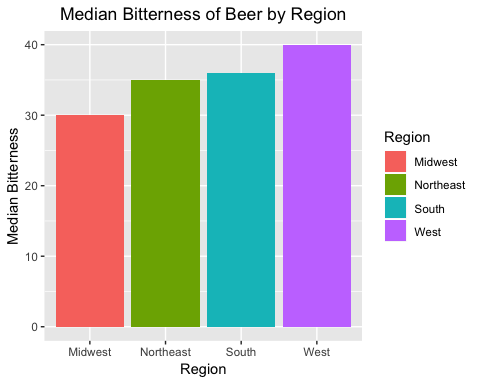
\includegraphics{BeerAnalysis_files/figure-latex/unnamed-chunk-17-1.pdf}

\begin{Shaded}
\begin{Highlighting}[]
\KeywordTok{ggplot}\NormalTok{(alcohol_and_bitterness_regionalized) }\OperatorTok{+}\StringTok{ }\KeywordTok{geom_col}\NormalTok{(}\KeywordTok{aes}\NormalTok{(Region, MedianAlcohol, }\DataTypeTok{fill =}\NormalTok{ Region)) }\OperatorTok{+}\StringTok{ }\KeywordTok{ggtitle}\NormalTok{(}\StringTok{"Median ABV of Beer by Region"}\NormalTok{) }\OperatorTok{+}\StringTok{ }\KeywordTok{ylab}\NormalTok{(}\StringTok{"Median Alcohol Content"}\NormalTok{) }\OperatorTok{+}\StringTok{ }\KeywordTok{theme}\NormalTok{(}\DataTypeTok{plot.title =} \KeywordTok{element_text}\NormalTok{(}\DataTypeTok{hjust =} \FloatTok{0.5}\NormalTok{))}
\end{Highlighting}
\end{Shaded}

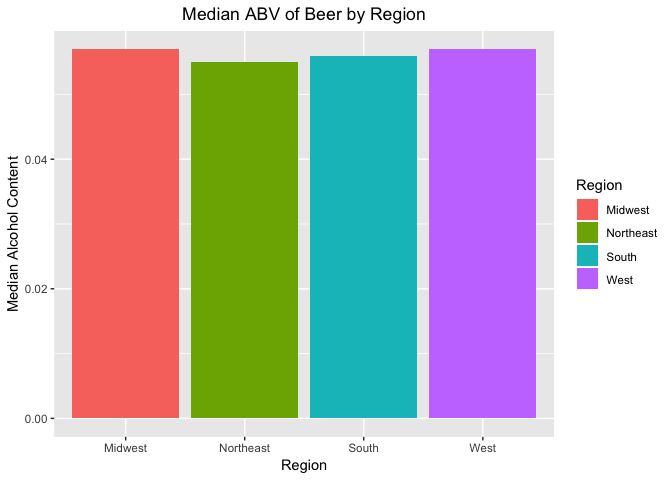
\includegraphics{BeerAnalysis_files/figure-latex/unnamed-chunk-17-2.pdf}

Median ABV values look constant by region, but some differences in
median bitterness (IBU) exists across region. Midwestern beers seem the
least bitter while Western beers are bitter by far.

\hypertarget{relationship-between-abv-and-ibu}{%
\subsubsection{Relationship between ABV and
IBU}\label{relationship-between-abv-and-ibu}}

Much discussion has been given to these beer characteristics above, but
is there any correlation between these variables? Here's a scatterplot
comparing them.

\begin{Shaded}
\begin{Highlighting}[]
\KeywordTok{ggplot}\NormalTok{(}\DataTypeTok{data=}\NormalTok{Brewtot, }\KeywordTok{aes}\NormalTok{(}\DataTypeTok{x=}\NormalTok{IBU, }\DataTypeTok{y=}\NormalTok{ABV)) }\OperatorTok{+}\KeywordTok{geom_point}\NormalTok{(}\DataTypeTok{shape =} \DecValTok{16}\NormalTok{, }\DataTypeTok{size =} \DecValTok{2}\NormalTok{, }\DataTypeTok{color=}\StringTok{"blue"}\NormalTok{) }\OperatorTok{+}\StringTok{ }\KeywordTok{stat_smooth}\NormalTok{(}\DataTypeTok{method =} \StringTok{'lm'}\NormalTok{, }\DataTypeTok{color=}\StringTok{'red'}\NormalTok{) }\OperatorTok{+}\StringTok{ }\KeywordTok{labs}\NormalTok{(}\DataTypeTok{title =} \StringTok{'Craft Beer IBU by ABV'}\NormalTok{) }\OperatorTok{+}\StringTok{ }\KeywordTok{theme}\NormalTok{(}\DataTypeTok{plot.title =} \KeywordTok{element_text}\NormalTok{(}\DataTypeTok{hjust =} \FloatTok{0.5}\NormalTok{))}
\end{Highlighting}
\end{Shaded}

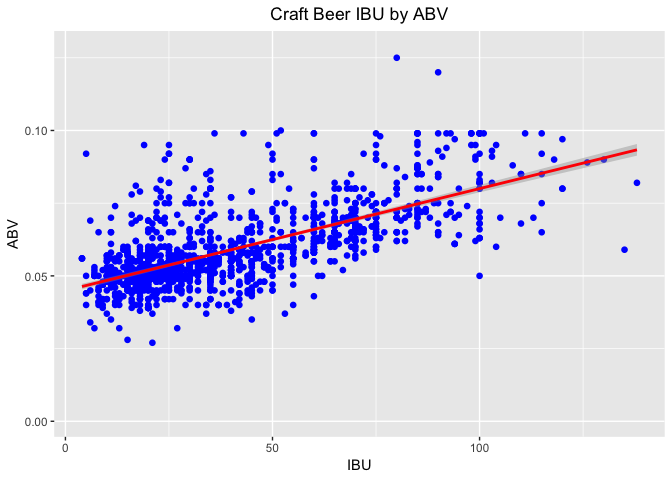
\includegraphics{BeerAnalysis_files/figure-latex/unnamed-chunk-18-1.pdf}

There is a moderate linear correlation. A Pearson correlation test
quantifies it.

\begin{Shaded}
\begin{Highlighting}[]
\KeywordTok{cor.test}\NormalTok{( }\OperatorTok{~}\StringTok{ }\NormalTok{ABV }\OperatorTok{+}\StringTok{ }\NormalTok{IBU,}\DataTypeTok{data=}\NormalTok{Brewtot,}\DataTypeTok{method =} \StringTok{"pearson"}\NormalTok{)}
\end{Highlighting}
\end{Shaded}

\begin{verbatim}

    Pearson's product-moment correlation

data:  ABV and IBU
t = 33.863, df = 1403, p-value < 2.2e-16
alternative hypothesis: true correlation is not equal to 0
95 percent confidence interval:
 0.6407982 0.6984238
sample estimates:
      cor 
0.6706215 
\end{verbatim}

At \emph{r} = 0.67, this is indeed moderate, but not strong, positive
correlation. The regression line illustrates that the variability may be
changing along the prediction line (heteroscedasticity). This
correlation does not show causation as the relationship may be affect by
third variables such as ingredients used, fermentation process, and
marketing needs.

\hypertarget{integrating-beer-consumption}{%
\subsubsection{Integrating Beer
Consumption}\label{integrating-beer-consumption}}

It's plausible to think that states with higher numbers of brewers or
beers have higher beer consumption. To investigate this assumption, 2018
\href{https://www.usatoday.com/story/money/personalfinance/2018/05/02/which-states-residents-drink-most-beer/569430002/}{data}
on total annual beer consumption (in gallons) by state is taken.

Note that the year for the \texttt{beer} and \texttt{brewers} data is
unknown, but we'll assume the general trend of data has not changed
significantly even if the data are a couple of years apart.

\begin{Shaded}
\begin{Highlighting}[]
\KeywordTok{library}\NormalTok{(rvest)}
\KeywordTok{library}\NormalTok{(stringr)}

\CommentTok{# scrape consumption info}
\NormalTok{scraping_beer <-}\StringTok{ }\KeywordTok{read_html}\NormalTok{(}\StringTok{"https://www.usatoday.com/story/money/personalfinance/2018/05/02/which-states-residents-drink-most-beer/569430002/"}\NormalTok{)}
\NormalTok{national_consum <-}\StringTok{ }\NormalTok{scraping_beer }\OperatorTok\StringTok{ }\KeywordTok{html_nodes}\NormalTok{(}\StringTok{"ul"}\NormalTok{) }\OperatorTok\StringTok{ }\KeywordTok{html_text}\NormalTok{() }\OperatorTok\StringTok{ }\KeywordTok{data.frame}\NormalTok{()}
\KeywordTok{colnames}\NormalTok{(national_consum)[}\DecValTok{1}\NormalTok{] <-}\StringTok{ "Total Consumption"}
\CommentTok{# remove first four rows (irrelevant info)}
\CommentTok{# use drop = FALSE since there's only 1 column}
\NormalTok{national_consum <-}\StringTok{ }\NormalTok{national_consum[}\OperatorTok{-}\KeywordTok{c}\NormalTok{(}\DecValTok{1}\OperatorTok{:}\DecValTok{4}\NormalTok{), , drop =}\StringTok{ }\OtherTok{FALSE}\NormalTok{]}
\CommentTok{# change column from factor to string (character)}
\NormalTok{national_consum}\OperatorTok{$}\StringTok{`}\DataTypeTok{Total Consumption}\StringTok{`}\NormalTok{ <-}\StringTok{ }\KeywordTok{as.character}\NormalTok{(national_consum}\OperatorTok{$}\StringTok{`}\DataTypeTok{Total Consumption}\StringTok{`}\NormalTok{)}

\NormalTok{beer_values =}\StringTok{ }\KeywordTok{c}\NormalTok{() }\CommentTok{# holds the actual consumption values}
\ControlFlowTok{for}\NormalTok{ (row }\ControlFlowTok{in}\NormalTok{ national_consum)\{}
\NormalTok{  total_consum <-}\StringTok{ }\KeywordTok{substring}\NormalTok{(row, }\DataTypeTok{first =} \KeywordTok{str_locate}\NormalTok{(row, }\StringTok{"Total"}\NormalTok{)[}\DecValTok{1}\NormalTok{], }\DataTypeTok{last =} \KeywordTok{str_locate}\NormalTok{(row, }\StringTok{"5 yr."}\NormalTok{)[}\DecValTok{1}\NormalTok{] }\OperatorTok{-}\StringTok{ }\DecValTok{1}\NormalTok{)}
\NormalTok{  total_consum_numeric <-}\StringTok{ }\KeywordTok{regmatches}\NormalTok{(total_consum, }\KeywordTok{regexpr}\NormalTok{(}\StringTok{'}\CharTok{\textbackslash{}\textbackslash{}}\StringTok{d+}\CharTok{\textbackslash{}\textbackslash{}}\StringTok{.+}\CharTok{\textbackslash{}\textbackslash{}}\StringTok{d'}\NormalTok{, total_consum)) }\OperatorTok\StringTok{ }\KeywordTok{as.numeric}\NormalTok{()}
\NormalTok{  beer_values <-}\StringTok{ }\KeywordTok{c}\NormalTok{(beer_values, total_consum_numeric)}
\NormalTok{\}}

\CommentTok{# make the beer values the column values of nationa_consum}
\NormalTok{national_consum}\OperatorTok{$}\StringTok{`}\DataTypeTok{Total Consumption}\StringTok{`}\NormalTok{ <-}\StringTok{ }\NormalTok{beer_values}
\CommentTok{# remove row names bc of improper numbering}
\KeywordTok{rownames}\NormalTok{(national_consum) <-}\StringTok{ }\OtherTok{NULL}


\CommentTok{# scrape the name of the states}
\NormalTok{statenames <-}\StringTok{ }\NormalTok{scraping_beer }\OperatorTok\StringTok{ }\KeywordTok{html_nodes}\NormalTok{(}\StringTok{"p"}\NormalTok{) }\OperatorTok\StringTok{ }\KeywordTok{html_text}\NormalTok{() }\OperatorTok\StringTok{ }\KeywordTok{data.frame}\NormalTok{()}
\CommentTok{# remove row names}
\KeywordTok{colnames}\NormalTok{(statenames)[}\DecValTok{1}\NormalTok{] <-}\StringTok{ 'State'}
\NormalTok{statenames}\OperatorTok{$}\NormalTok{State <-}\StringTok{ }\KeywordTok{as.character}\NormalTok{(statenames}\OperatorTok{$}\NormalTok{State)}
\KeywordTok{rownames}\NormalTok{(statenames) <-}\StringTok{ }\OtherTok{NULL}
\CommentTok{# immediately delete irrelevant first 22 and last 4 rows}
\NormalTok{statenames <-}\StringTok{ }\NormalTok{statenames[}\OperatorTok{-}\KeywordTok{c}\NormalTok{(}\DecValTok{1}\OperatorTok{:}\DecValTok{22}\NormalTok{, }\DecValTok{88}\OperatorTok{:}\DecValTok{91}\NormalTok{), }\DecValTok{1}\NormalTok{, drop =}\StringTok{ }\OtherTok{FALSE}\NormalTok{]}
\CommentTok{# first isolate rows similar in format to "46. New York"}
\NormalTok{statenames <-}\StringTok{ }\NormalTok{statenames[}\KeywordTok{grepl}\NormalTok{(}\StringTok{"}\CharTok{\textbackslash{}\textbackslash{}}\StringTok{d+}\CharTok{\textbackslash{}\textbackslash{}}\StringTok{."}\NormalTok{, statenames}\OperatorTok{$}\NormalTok{State), , drop =}\StringTok{ }\OtherTok{FALSE}\NormalTok{]}
\CommentTok{# remove list numbers and "(tied)"}
\NormalTok{statenames}\OperatorTok{$}\NormalTok{State <-}\StringTok{ }\KeywordTok{str_replace_all}\NormalTok{(statenames}\OperatorTok{$}\NormalTok{State, }\StringTok{"}\CharTok{\textbackslash{}\textbackslash{}}\StringTok{d+}\CharTok{\textbackslash{}\textbackslash{}}\StringTok{.|}\CharTok{\textbackslash{}\textbackslash{}}\StringTok{(+tied+}\CharTok{\textbackslash{}\textbackslash{}}\StringTok{)"}\NormalTok{, }\StringTok{""}\NormalTok{)}
\CommentTok{# remove spaces before or after name}
\NormalTok{statenames}\OperatorTok{$}\NormalTok{State <-}\StringTok{ }\KeywordTok{str_replace_all}\NormalTok{(statenames}\OperatorTok{$}\NormalTok{State, }\StringTok{"^}\CharTok{\textbackslash{}\textbackslash{}}\StringTok{s|}\CharTok{\textbackslash{}\textbackslash{}}\StringTok{s$"}\NormalTok{, }\StringTok{""}\NormalTok{)}
\KeywordTok{rownames}\NormalTok{(statenames) <-}\StringTok{ }\OtherTok{NULL}
\CommentTok{# convert to abbreviations using state.name and state.abb built-ins}
\ControlFlowTok{for}\NormalTok{ (i }\ControlFlowTok{in} \DecValTok{1}\OperatorTok{:}\KeywordTok{nrow}\NormalTok{(statenames)) \{}
\NormalTok{  statenames}\OperatorTok{$}\NormalTok{State[i] <-}\StringTok{ }\NormalTok{state.abb[}\KeywordTok{grep}\NormalTok{(statenames}\OperatorTok{$}\NormalTok{State[i], state.name)]}
\NormalTok{\}}
\CommentTok{# merge statenames and national_consum to a unified dataset}
\NormalTok{national_consum <-}\StringTok{ }\KeywordTok{cbind}\NormalTok{(national_consum, statenames)}
\CommentTok{#merge national_consum and beer_landscape for the total dataset}
\NormalTok{complete_beer_landscape <-}\StringTok{ }\KeywordTok{merge}\NormalTok{(national_consum, beer_landscape, }\DataTypeTok{by =} \StringTok{'State'}\NormalTok{) }\OperatorTok
\StringTok{  }\KeywordTok{arrange}\NormalTok{(}\KeywordTok{desc}\NormalTok{(}\StringTok{`}\DataTypeTok{Total Consumption}\StringTok{`}\NormalTok{))}
\KeywordTok{colnames}\NormalTok{(complete_beer_landscape)[}\DecValTok{4}\NormalTok{] <-}\StringTok{ "Total Brewers"}
\CommentTok{# format table}
\KeywordTok{kable}\NormalTok{(complete_beer_landscape, }\DataTypeTok{align =} \KeywordTok{rep}\NormalTok{(}\StringTok{'c'}\NormalTok{,}\DecValTok{4}\NormalTok{)) }\OperatorTok\StringTok{ }\KeywordTok{kable_styling}\NormalTok{(}\DataTypeTok{bootstrap_options =} \StringTok{"striped"}\NormalTok{, }\DataTypeTok{full_width =}\NormalTok{ F)}
\end{Highlighting}
\end{Shaded}

\begin{table}[H]
\centering
\begin{tabular}{c|c|c|c}
\hline
State & Total Consumption & Beers & Total Brewers\\
\hline
CA & 724.9 & 183 & 39\\
\hline
TX & 626.3 & 130 & 28\\
\hline
FL & 423.1 & 58 & 15\\
\hline
NY & 327.5 & 74 & 16\\
\hline
IL & 259.4 & 91 & 18\\
\hline
PA & 254.1 & 100 & 25\\
\hline
OH & 234.7 & 49 & 15\\
\hline
NC & 188.0 & 59 & 19\\
\hline
MI & 186.7 & 162 & 32\\
\hline
GA & 179.6 & 16 & 7\\
\hline
VA & 152.7 & 40 & 16\\
\hline
WI & 147.1 & 87 & 20\\
\hline
NJ & 138.0 & 8 & 3\\
\hline
AZ & 135.6 & 47 & 11\\
\hline
WA & 135.6 & 68 & 23\\
\hline
MO & 125.6 & 42 & 9\\
\hline
MA & 121.9 & 82 & 23\\
\hline
TN & 120.8 & 6 & 3\\
\hline
CO & 117.6 & 265 & 47\\
\hline
MN & 115.4 & 55 & 12\\
\hline
SC & 115.0 & 14 & 4\\
\hline
IN & 112.7 & 139 & 22\\
\hline
AL & 103.7 & 10 & 3\\
\hline
LA & 99.4 & 19 & 5\\
\hline
OR & 95.4 & 125 & 29\\
\hline
MD & 90.1 & 21 & 7\\
\hline
KY & 77.1 & 21 & 4\\
\hline
NV & 72.9 & 11 & 2\\
\hline
IA & 72.0 & 30 & 5\\
\hline
OK & 70.7 & 19 & 6\\
\hline
MS & 66.6 & 11 & 2\\
\hline
CT & 54.2 & 27 & 8\\
\hline
KS & 53.2 & 23 & 3\\
\hline
AR & 52.0 & 5 & 2\\
\hline
NE & 45.3 & 25 & 5\\
\hline
NM & 43.8 & 14 & 4\\
\hline
NH & 41.8 & 8 & 3\\
\hline
UT & 38.1 & 26 & 4\\
\hline
WV & 37.8 & 2 & 1\\
\hline
ME & 34.9 & 27 & 9\\
\hline
ID & 31.5 & 30 & 5\\
\hline
MT & 30.8 & 40 & 9\\
\hline
HI & 30.6 & 27 & 4\\
\hline
SD & 23.7 & 7 & 1\\
\hline
ND & 20.9 & 3 & 1\\
\hline
DE & 20.7 & 2 & 2\\
\hline
RI & 18.4 & 27 & 5\\
\hline
VT & 15.6 & 27 & 10\\
\hline
AK & 14.0 & 25 & 7\\
\hline
WY & 12.3 & 15 & 4\\
\hline
\end{tabular}
\end{table}

California, Texas, and Florida are the top three beer consuming states.

Here's a plot displaying the relationship between consumption and number
of brewers.

\begin{Shaded}
\begin{Highlighting}[]
\KeywordTok{ggplot}\NormalTok{(complete_beer_landscape) }\OperatorTok{+}\StringTok{ }\KeywordTok{geom_point}\NormalTok{(}\KeywordTok{aes}\NormalTok{(}\StringTok{`}\DataTypeTok{Total Brewers}\StringTok{`}\NormalTok{, }\StringTok{`}\DataTypeTok{Total Consumption}\StringTok{`}\NormalTok{), }\DataTypeTok{col =} \StringTok{'purple'}\NormalTok{ )}\OperatorTok{+}\KeywordTok{ggtitle}\NormalTok{(}\StringTok{"Comparing Beer Consumption Levels to Number of Breweries"}\NormalTok{) }\OperatorTok{+}\StringTok{ }\KeywordTok{xlab}\NormalTok{(}\StringTok{"Total Brewers"}\NormalTok{) }\OperatorTok{+}\StringTok{ }\KeywordTok{ylab}\NormalTok{(}\StringTok{"Total Consumption (Gallons)"}\NormalTok{) }\OperatorTok{+}\StringTok{ }\KeywordTok{theme}\NormalTok{(}\DataTypeTok{plot.title =} \KeywordTok{element_text}\NormalTok{(}\DataTypeTok{hjust =} \FloatTok{0.5}\NormalTok{))}
\end{Highlighting}
\end{Shaded}

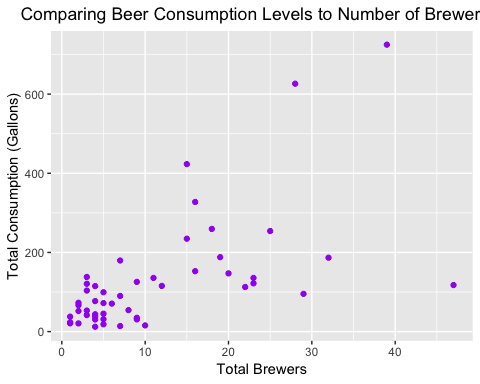
\includegraphics{BeerAnalysis_files/figure-latex/unnamed-chunk-21-1.pdf}

This confirms the idea that states with more brewers tend to drink more
beer. A notable exception is Colorado, the state with a
disproportionately high number of brewers but low overall consumption.

\begin{Shaded}
\begin{Highlighting}[]
\NormalTok{complete_beer_landscape[}\KeywordTok{which}\NormalTok{(complete_beer_landscape}\OperatorTok{$}\StringTok{`}\DataTypeTok{Total Brewers}\StringTok{`} \OperatorTok{>}\StringTok{ }\DecValTok{40}\NormalTok{), ]}
\end{Highlighting}
\end{Shaded}

\begin{verbatim}
   State Total Consumption Beers Total Brewers
19    CO             117.6   265            47
\end{verbatim}

\hypertarget{conclusion}{%
\subsubsection{Conclusion}\label{conclusion}}

To maximize potential it is advisable to build breweries in states with
few breweries but moderately high beer consumption. Examples of such
states include New Jersey, Tennessee, and South Carolina.

With Tennessee, we can experiment with a more bitter beer with a
flavorful raspberry twist. Call it the `Tarty Tennesseean'. An inital
goal (a more conservative estimate) would be gaining at least 40\%
regional adoption within five years.


\end{document}
